\documentclass{article}

\usepackage[utf8]{inputenc}
\usepackage[greek, british]{babel}
\usepackage{alphabeta}
\usepackage{libertine}
\usepackage{csquotes}
\usepackage[backend=biber, sorting=none]{biblatex}
\usepackage{hyperref}
\usepackage{graphicx}
\usepackage{float}
\graphicspath{ {./images/} }

\pagenumbering{arabic}

\addbibresource{refs.bib}

\newcommand{\code}{\texttt}

\title{Documentation for Numpy Classifiers}

\begin{document}
	
\maketitle


\section{Project Structure}
The project is divided into 3 modules, containing a total of 10 python source code files. 

The \code{lib} module contains shared code between the models, running scripts and tests and includes:
\begin{itemize}
	\item \code{load\_mnist.py}, which performs data loading and pre-processing 
	\item \code{common.py}, which contains common math functions for the above primitives
\end{itemize}

The \code{models} module contains our models and includes:
\begin{itemize}
	\item \code{logistic\_regression.py}, which contains the logistic regression model
	\item \code{mlp.py}, which contains the MLP neural network model 
	\item \code{sgd.py}, which contains the neural network model variation using batch stochastic gradient descent
\end{itemize}

The \code{test} module contains files used to verify the model's behaviors:
\begin{itemize}
	\item \code{gradcheck.py}, which tests  the back-propagation algorithm used in the two MLP models
	\item \code{test\_load\_mnist.py} which helps validate our data
\end{itemize}

Finally, the \code{run} module contains scripts used to generate the graphs and results of this document. It includes:
\begin{itemize}
		\item \code{run\_logistic.py}
		\item \code{run\_mlp.py}
		\item \code{run\_sgd.py}
\end{itemize}


Full documentation of the code and implementation can be found in the above files in the form of python docstrings and comments.


\section{Logistic Regression}

Our classifier has been implemented in the file \code{logistic\_regression.py}.

The code to run the model is in the file \code{run\_logistic.py}. We will run the model with hyperparameters \code{iter = 500} and \code{alpha = 0.2}. The result is that the training accuracy is equal to $0.982$ and the test accuracy is equal to $0.981$. The full results of training and testing are shown in Figure \ref{logistic_train_test}.

\begin{figure}
	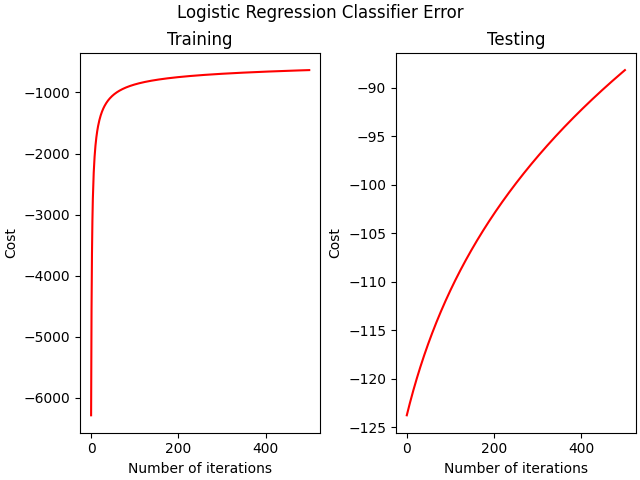
\includegraphics[width=7cm]{logistic_error.png}
	\centering
	\caption{The results of training and testing on our classifier. Left: The training cost as a function of the iterations of the gradient ascent algorithm. Right: The corresponding testing cost. Recall that the scales of the graphs are not equal, as the already trained classifier starts with a much lower cost. }
	\label{logistic_train_test}
\end{figure}


The code to produce the above graphs and results is in the file \code{run\_logistic.py}.

We choose our interval of \code{$³lambda$} values logarithmically, since the optimal normalization value is much more likely to be fairly close to 0. Logarithmic scaling allows us to search more values of \code{$³lambda$} the closer we get to our lower search limit, $10^{-4}$. This approach is also used in practice for normalization $L_{2}$ \cite{jerome}.

We note that due to computational requirements, the number of iterations of our models is reduced to 250 iterations. During the execution of the program there is also a possibility that warnings for numerical overflow may occur, which we have disabled. This is a result of choosing too large a value of \code{$\lambda$}, mostly in the interval [8, 10]. At this point the normalization is so strong that it prevents our model from learning, and so it guesses the same class for each control example.

In our case, the model prefers the minimum normalization value \code{$lambda = 10^{-4}$} with a control accuracy of $0.981$. 

We observe that the test accuracy with the chosen value \code{$lambda$} is lower than the one with no regularization. This suggests either that the optimal value is outside (and more precisely before) our search space, or that the statistical error is responsible for the difference.

The full search results for the hyper parameter are shown in Figure \ref{logistic_lambda_accuracy}.

\begin{figure}
	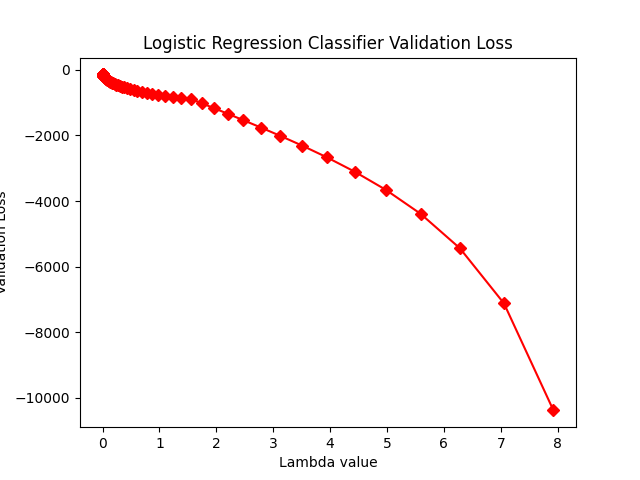
\includegraphics[width=7cm]{logistic_lambda_accuracy.png}
	\centering
	\caption{ The results of the search for the optimal \code{$_lambda$}. The diamonds represent the values we examined. Notice the number of values examined at the beginning compared to the end of our search field}.
	\label{logistic_lambda_accuracy}
\end{figure}


\section{Shallow Neural Network}


Our neural network has been implemented in the \code{mlp.py} file. It consists of two weight matrices and two bias matrices:

\begin{itemize}
	\item The table \code{h\_w} (hidden weights) has size $IxH$
	\item The table \code{o\_w} (output weights) has size $HxO$
	\item The table \code{h\_b} (hidden bias) has size $1xH$
	\item The table \code{o\_b} (output bias) has size $1xO$
\end{itemize}

where I= \code{input\_size}, H= \code{hidden\_layer\_size}, O= \code{output\_size}. The code to run the network is in the \code{run\_mlp.py} file, which also executes code for queries H, I.

We will run the model with hyper-parameters \code{m=2}, \code{$eta$=0.2} and \code{tolerance=0.001}. The \code{tolerance} is a necessary hyper parameter for the early stopping algorithm, which determines how much the loss must have been reduced for the current season to be considered an "improvement". The result is that the training accuracy is equal to $0.977$, the average validation cost is equal to $0.0634$, the control accuracy is equal to $0.975$, and the average testing cost is equal to $0.0753$. The full training results are shown in Figure \ref{mlp_train_test}.

\begin{figure}
	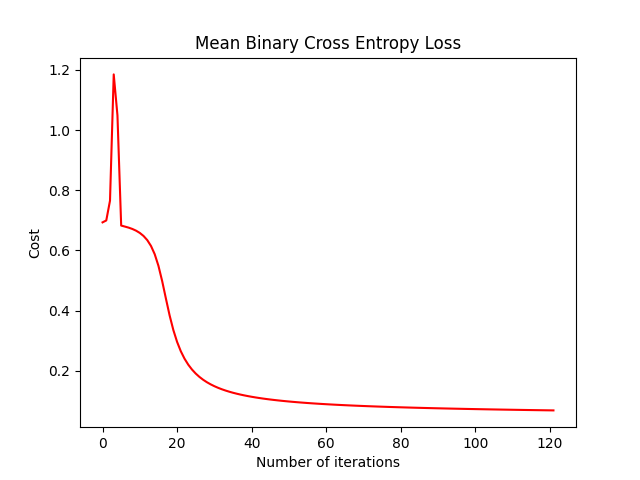
\includegraphics[width=10cm]{mlp_error.png}
	\centering
	\caption{The training cost as a function of the number of iterations of the gradient descent algorithm.}
	\label{mlp_train_test}
\end{figure}

We perform a grid search for the parameters $m, \eta$. We choose our interval of $\eta$ values in the search space $[0.5, 10^{-5}]$, exponentially close to $0.5$ since we empirically expect its optimal value to be close to $0.5, 0.01, 0.01$. The result for this network is $(\eta=0.5, m=4, E=139)$ with an average control cost equal to $0.0669$ and a testing accuracy of $0.981$.

The grid search runtime can be found in the file \code{run\_mlp.py}. The search takes about 20 minutes to get the optimal combination of hyper-parameters, which is almost entirely due to training and verifying models with $M \in \{256, 512, 1024\}$. 

We use the \code{predict} method of our model to obtain its predicted labels. In the test set, the model with the optimized parameters achieves a control accuracy equal to $0.979$ and a testing cost equal to $0.0569$.

\section{Batch Stochastic Gradient Descent}
The SGD classifier can be found in the \code{sgd.py} file.

We implement the stochastic downward gradient classifier as a subclass of our previous classifier. The main change is passing mini-batches to the \code{back\_propagation} method instead of the set of training samples. Specifically, instead of passing a 9072x784 matrix to \code{back\_propagation}, we pass a 9072x784 matrix Bx784 where B is the size of the mini-batch. The training examples and their labels are shuffled before each iteration of the algorithm so that our model considers a different set of examples each time. The method itself remains the same.
	
The execution program for the classifier and the grid search below can be found in the \code{run\_sgd.py} file. Running our classifier with similar parameters to the previous one and with an arbitrary mini-batch size=128 achieves a training accuracy of $0.976$ at a cost of $0.0678$ and a testing accuracy of $0.977$ at a cost of $0.0793$. This accuracy is slightly worse than the logistic regression classifier, although due to the mini-batch computation and the early-stopping criterion, the model is significantly faster.
	
A complete graph of the evolution of the training loss can be found in Figure \ref{sgd_train_test}. We observe that our classifier cost follows the same path as that of Figure \ref{mlp_train_test}, albeit bumpier. This is due to the randomness of the SGD algorithm, which adds "noise" to the training process through the random and limited amount of data our model sees in each iteration of SGD.

\begin{figure}[H].
	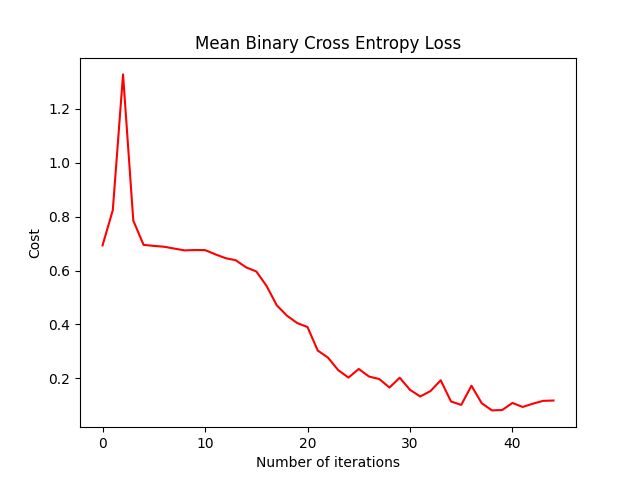
\includegraphics[width=7cm]{sgd_error.png}
	\centering
	\caption{The training cost as a function of the iterations of the stochastic gradient descent algorithm.}
	\label{sgd_train_test}
\end{figure}

Testing our model with values $B=2^{i}, i=1,2,...,8$, the optimal mini-batch size value appears to be $B=256$, with a validation cost equal to $0.6877$ and with $E=16$ training epochs. Running our model on the control set yields test cost equal to $0.0864$ and a testing accuracy equal to $0.970$.

Using the optimal value B, we can run the same method to search for optimal hyper-parameters as in question H. Using the same methodology and the same hyper-parameter search space, our program finds optimal hyper-parameters $(\eta=0.139, m=4, E=103)$ with an average validation cost equal to $0.0735$. Running our model on the control set yields a validation cost equal to $0.0758$ and a validation accuracy equal to $0.979$.

\textit{Please note that due to the randomness of the SGD algorithm, the results of the run may be different from those reported in this document. There is also a possibility of gradient vanishing for small values of B.}	


\printbibliography

\end{document}